\section{User Evaluation Test Instructions}
\label{app-userEval}
The purpose of this test is to construct the fuzzy logic tipper example, in three different software systems, so that the strengths and weaknesses of each of these systems can be identified. The tipper example is a simple fuzzy system that uses food quality (rated from 0 to 10) and service quality (rated from 0 to 10) as inputs, to determine how much of a tip should be left (between 0 and 30 percent). \ \\
\ \\
Please follow the instructions below, and do not hesitate to ask for help if you are stuck, this is an evaluation of the user interface, and not of you. After each step, please explain your thought process, and how you found the task.

\begin{enumerate}
\item (\textbf{FuzzyToolkitUoN only}) Create a new \textbf{Fuzzy Inference System}
\item Add a new \textbf{input variable}, called \textbf{Service}, with range \textbf{0} to \textbf{10}
\item Add the following \textbf{membership functions} to the \textbf{Service} variable
	\begin{enumerate}
	\item A \textbf{Gaussian} function, named \textbf{Poor}, with parameters:\\
	\begin{tabular}{ll}
	Sigma 	& 1.5 \\
	Mean	& 0   \\
	Height	& 1   \\
	\end{tabular}
	\item A \textbf{Gaussian} function, named \textbf{Good}, with parameters:\\
	\begin{tabular}{ll}
	Sigma 	& 1.5 \\
	Mean	& 5   \\
	Height	& 1   \\
	\end{tabular}	
	\item A \textbf{Gaussian} function, named \textbf{Excellent}, with parameters:\\
	\begin{tabular}{ll}
	Sigma 	& 1.5 \\
	Mean	& 10   \\
	Height	& 1   \\
	\end{tabular}	
	\end{enumerate}
\item Add a new \textbf{input variable}, called \textbf{Food}, with range \textbf{0} to \textbf{10}	
\item Add the following \textbf{membership functions} to the \textbf{Food} variable
	\begin{enumerate}
	\item A \textbf{Trapezoidal} function, named \textbf{Rancid}, with parameters:\\
	\begin{tabular}{ll}
	Left Foot 		& 0		\\
	Left Shoulder 	& 0		\\
	Right Shoulder 	& 1		\\
	Right Foot 		& 3		\\
	Height			& 1   	\\
	\end{tabular}
	\item A \textbf{Trapezoidal} function, named \textbf{Delicious}, with parameters:\\
	\begin{tabular}{ll}
	Left Foot 		& 7		\\
	Left Shoulder 	& 9		\\
	Right Shoulder 	& 10	\\
	Right Foot 		& 10	\\
	Height			& 1   	\\
	\end{tabular}		
	\end{enumerate}
\newpage 
\item Add a new \textbf{output variable}, called \textbf{Tip}, with range \textbf{0} to \textbf{30}	
\item Add the following \textbf{membership functions} to the \textbf{Tip} variable
	\begin{enumerate}
	\item A \textbf{Triangular} function, named \textbf{Cheap}, with parameters:\\
	\begin{tabular}{ll}
	Left  			& 0		\\
	Mean 			& 5		\\
	Right 			& 10		\\
	Height			& 1   	\\
	\end{tabular}
	\item A \textbf{Triangular} function, named \textbf{Average}, with parameters:\\
	\begin{tabular}{ll}
	Left  			& 10		\\
	Mean 			& 15		\\
	Right 			& 20		\\
	Height			& 1   	\\
	\end{tabular}	
	\item A \textbf{Triangular} function, named \textbf{Generous}, with parameters:\\
	\begin{tabular}{ll}
	Left  			& 20		\\
	Mean 			& 25		\\
	Right 			& 30		\\
	Height			& 1   	\\
	\end{tabular}			
	\end{enumerate}	
\item Add the following \textbf{rules} to the system
	\begin{enumerate}
	\item IF Service is Poor OR Food is Rancid, Then Tip is Cheap (Weight 1)
	\item IF Service is Average, Then Tip is Average (Weight 1)
	\item IF Service is Excellent OR Food is Delicious, Then Tip is Generous (Weight 1)
	\end{enumerate}
\item (\textbf{FuzzyToolkitUoN, and o-Fuzz only}) Please evaluate the following values:
	\begin{enumerate}
	\item Service score of 0, Food score of 0
	\item Service score of 10, Food score of 10
	\end{enumerate}
\item Please change the \textbf{defuzzification method}	of the system to \textbf{Bisector}
\item \textbf{Save} the inference system as a file to your hard drive
\item Now, read that same file back into the system
\end{enumerate}

\newpage
\section{Table of Results of User Evaluation}
\label{app-torous}



\begin{center}
\begin{tabular}{cccc}
\hline
\textbf{Group} 	& \textbf{\# of Members} & \textbf{Fuzzy Logic Skill} & \textbf{Computer Skill} \\
\hline
1				& 7 						 & Low			& Low		\\	
2				& 5  						 & Low			& High		\\
3				& 3 						 & High			& Low 		\\
4				& 8 						 & High 		& High		\\
\hline
\end{tabular}
\end{center}

\noindent 
This table lists the time taken (in Minutes) for each participant to complete each task of the expirement. Task 1 was to follow the instruction list using FuzzyToolkitUoN, Task 2 was to follow the instruction list using the MATLAB Fuzzy Toolbox and Task 3 was to follow the instruction list using the new project created in this report. It also details the participants favourite, and least favourite software, of the three (OF standing for O-Fuzz, this project, FTU standing for FuzzyToolkitUoN, and M standing for MATLAB's fuzzy toolbox).\ \\
\begin{changemargin}{-1cm}{-1cm}
\begin{tabular}{ccccccc}
\hline
Participant	&	Group	&	Task 1	&	Task 2	&	Task 3	&	Most Liked Software	&	Least Liked Software 	\\
\hline
1			&	1		&	53		&	21		&	14		&	OF					&	FTU						\\	
2			&	1		&	45		&	23		&	15		&	OF					&	FTU						\\
3			&	1		&	61		&	34		&	20		&	OF					&	FTU						\\	
4			&	1		&	70		&	36		&	21		&	M					&	FTU						\\	
5			&	1		&	63		&	31		&	15		&	OF					&	FTU						\\		
6			&	1		&	53		&	23		&	13		&	M					&	FTU						\\	
7			&	1		&	54		&	26		&	16		&	OF					&	FTU						\\	
8			&	2		&	35		&	13		&	9		&	OF					&	FTU						\\		
9			&	2		&	25		&	14		&	8		&	M					&	FTU						\\	
10			&	2		&	27		&	15		&	10		&	OF					&	FTU						\\			
11			&	2		&	26		&	11		&	11		&	OF					&	FTU						\\		
12			&	2		&	31		&	14		&	10		&	M					&	FTU						\\		
13			&	3		&	33		&	16		&	9		&	M					&	FTU						\\	
14			&	3		&	30		&	16		&	10		&	OF					&	FTU						\\			
15			&	3		&	40		&	33		&	13		&	OF					&	FTU						\\			
16			&	4		&	14		&	11		&	4 		&	OF					&	FTU						\\		
17			&	4		&	28		&	12		&	6 		&	OF					&	FTU						\\			
18			&	4		&	20		&	10		&	6 		&	M					&	FTU						\\	
19			&	4		&	21		&	12		&	5 		&	OF					&	FTU						\\			
20			&	4		&	12		&	13		&	6 		&	FTU					&	M 						\\			
21			&	4		&	25		&	10		&	4 		&	OF					&	FTU						\\		
22			&	4 		&	18		&	14		&	5 		&	OF					&	FTU						\\
23			&	4 		&	16		&	11		&	5 		&	M					&	FTU						\\
\hline
\end{tabular}			
\end{changemargin}
\newpage 
\section{Complete Test Listing}
\label{app-ctl}
\begin{longtable}{p{5cm}|p{6cm}|p{3cm}}
\hline 
\textbf{Test} & \textbf{Expected Results} & \textbf{Actual Results} \\
\hline 
Users will be able to create Gaussian membership functions 
& There will be an option to specify a Gaussian membership function
& As expected \\ 
\hline
  \multicolumn{3}{c}{
  \fbox{ \raisebox{-\totalheight}{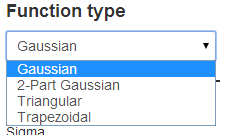
\includegraphics[width=0.3\textwidth]{images/test1.png}} }}\\
  \multicolumn{3}{l}{ }     \\\hline
Users will be able to create 2-Part Gaussian membership functions 
& There will be an option to specify a 2-Part Gaussian membership function
& As expected \\ 
\hline
  \multicolumn{3}{c}{
  \fbox{ \raisebox{-\totalheight}{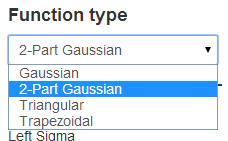
\includegraphics[width=0.3\textwidth]{images/test1-a.png}} }}\\
 \multicolumn{3}{l}{ }     \\\hline
Users will be able to create Triangular membership functions 
&There will be an option to specify specify a Triangular membership function
& As expected \\ 
\hline
  \multicolumn{3}{c}{
  \fbox{ \raisebox{-\totalheight}{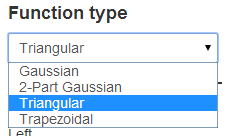
\includegraphics[width=0.3\textwidth]{images/test1-b.png}} }}\\
 \multicolumn{3}{l}{ }     \\\hline
Users will be able to create Trapezoidal membership functions 
& There will be an option to specify a Trapezoidal membership function
& As expected \\ 
\hline
  \multicolumn{3}{c}{
  \fbox{ \raisebox{-\totalheight}{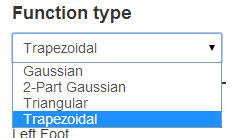
\includegraphics[width=0.3\textwidth]{images/test1-c.png}} }}\\
 \multicolumn{3}{l}{ }     \\








\hline Users will be able to add membership functions to variables 

& There will be a button to add membership functions to variables 

& As expected \\ 
  \hline
 \multicolumn{3}{c}{ \raisebox{-\totalheight}{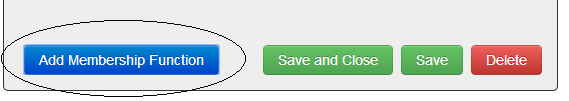
\includegraphics[width=0.5\textwidth]{images/test2.png}} }\\ 
 \multicolumn{3}{l}{ }     \\\hline

Users will be able edit membership function names 
& There will be a ``function name'' parameter box 
& As Expected \\ 
  \hline
 \multicolumn{3}{c}{
 \fbox{ \raisebox{-\totalheight}{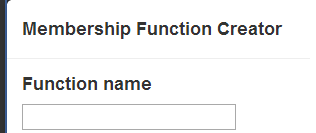
\includegraphics[width=0.3\textwidth]{images/test4.png}} }}\\ 
 \multicolumn{3}{l}{ }     \\\hline

Users will be able edit membership function parameters 
& There will be input boxes to specify function parameters 
& As Expected \\ 
  \hline
 \multicolumn{3}{c}{\fbox{ \raisebox{-\totalheight}{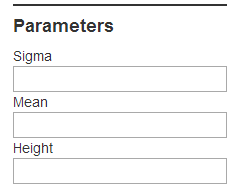
\includegraphics[width=0.3\textwidth]{images/test5.png}} }}\\ 
 \multicolumn{3}{l}{ }     \\\hline

Users will be able to delete membership functions from variables 
&  Each function will have a delete button
& As Expected \\ 
  \hline
 \multicolumn{3}{c}{ \raisebox{-\totalheight}{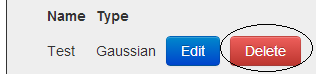
\includegraphics[width=0.5\textwidth]{images/test3.png}} }\\ 
 \multicolumn{3}{l}{ }     \\\hline

Users will be able to access help on how to create membership functions 
& There will be a show help button, that when pressed, will display an explanation of the window & 
As Expected\\ 
  \hline
 \multicolumn{3}{c}{ \raisebox{-\totalheight}{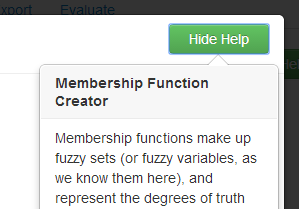
\includegraphics[width=0.3\textwidth]{images/test6.png}} }\\ 
 \multicolumn{3}{l}{ }     \\\hline

Users will be able to see a plot of their membership functions 
&  A plot of the membership function will be displayed after all parameters have been given
& As Expected\\ 
  \hline
 \multicolumn{3}{c}{ \raisebox{-\totalheight}{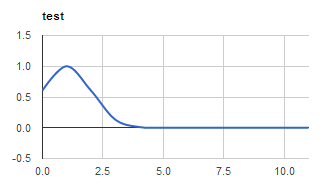
\includegraphics[width=0.4\textwidth]{images/test7.png}} }\\ 
 \multicolumn{3}{l}{ }     \\\hline

Users will be able to create input linguistic variables 
& There will be an ``inputs'' tab, with an ``Add New Variable'' button
& As Expected \\ 
  \hline
 \multicolumn{3}{c}{
 \fbox{ \raisebox{-\totalheight}{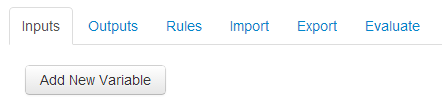
\includegraphics[width=0.5\textwidth]{images/test8.png}} }}\\ 
 \multicolumn{3}{l}{ }     \\\hline

Users will be able to create output linguistic variables& There will be an ``outputs'' tab, with an ``Add New Variable'' button
& As Expected \\  
  \hline
 \multicolumn{3}{c}{\fbox{ \raisebox{-\totalheight}{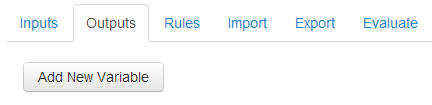
\includegraphics[width=0.5\textwidth]{images/test9.png}} }}\\ 
 \multicolumn{3}{l}{ }     \\\hline

Users will be able to edit the range of linguistic variables 
& There will be input boxes for both minimum and maximum range
& As Expected \\ 
  \hline
 \multicolumn{3}{c}{ \raisebox{-\totalheight}{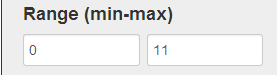
\includegraphics[width=0.3\textwidth]{images/test11.png}} }\\ 
 \multicolumn{3}{l}{ }     \\\hline

Users will be able to delete variables & There will be a button that deletes variables & As Expected \\ 
  \hline
 \multicolumn{3}{c}{ \raisebox{-\totalheight}{
\includegraphics[width=0.5\textwidth]{images/test12.png}} }\\ 
 \multicolumn{3}{l}{ }     \\\hline

Users will be able to rename variables & There will be an input box to change the name of a variable & As Expected \\ 
  \hline
 \multicolumn{3}{c}{ \raisebox{-\totalheight}{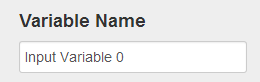
\includegraphics[width=0.3\textwidth]{images/test13.png}} }\\ 
 \multicolumn{3}{l}{ }     \\\hline

Users will be able to access help on how to create variables &  There will be a show help button, that when pressed, will display an explanation of the page  & As Expected  \\ 
  \hline
 \multicolumn{3}{c}{\fbox{ \raisebox{-\totalheight}{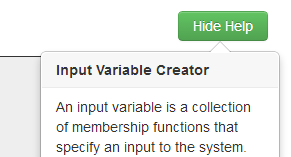
\includegraphics[width=0.3\textwidth]{images/test14.png}} }}\\ 
 \multicolumn{3}{l}{ }     \\\hline

Users will be able to create rules for the system & There will be an ``Add New Rule'' button on the Rules page & As Expected \\ 
  \hline
 \multicolumn{3}{c}{\fbox{ \raisebox{-\totalheight}{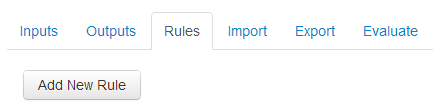
\includegraphics[width=0.45\textwidth]{images/test15.png}} }}\\ 
 \multicolumn{3}{l}{ }     \\\hline

Users will be able to specify rule terms & There will be dropdown boxes for each variable in the system, that users can select terms from & As Expected \\ 
  \hline
 \multicolumn{3}{c}{ \raisebox{-\totalheight}{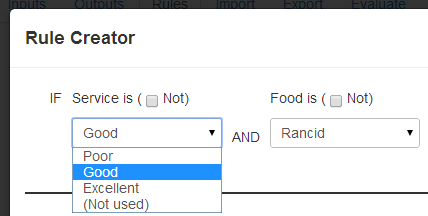
\includegraphics[width=0.4\textwidth]{images/test16.png}} }\\ 
 \multicolumn{3}{l}{ }     \\\hline

Users will be able to negate certain terms in a rule & There will be a checkbox above each term, symbolising negation & As Expected \\ 
  \hline
 \multicolumn{3}{c}{\fbox{ \raisebox{-\totalheight}{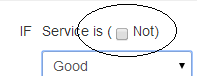
\includegraphics[width=0.25\textwidth]{images/test17.png}} }}\\ 
 \multicolumn{3}{l}{ }     \\\hline

Users will be able to change the weight of a rule & There will be a slider, and input box, to change the rule weight & As Expected \\ 
  \hline
 \multicolumn{3}{c}{\fbox{ \raisebox{-\totalheight}{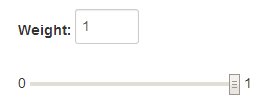
\includegraphics[width=0.4\textwidth]{images/test18.png}} }}\\ 
 \multicolumn{3}{l}{ }     \\\hline

Users will be able to specify the connective to be used in the rule & There will be a set of radio buttons to toggle between connectives & As Expected  \\ 
  \hline
 \multicolumn{3}{c}{\fbox{ \raisebox{-\totalheight}{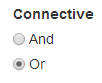
\includegraphics[width=0.2\textwidth]{images/test19.png}} }}\\ 
 \multicolumn{3}{l}{ }     \\\hline

Users will be able to edit any previously constructed rules & There will be an edit button aside each constructed rule & As Expected \\ 
  \hline
 \multicolumn{3}{c}{\fbox{ \raisebox{-\totalheight}{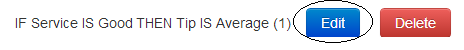
\includegraphics[width=0.45\textwidth]{images/test20.png}} }}\\ 
 \multicolumn{3}{l}{ }     \\\hline

Users will be able to delete any previously constructed rules & There will be a  delete button aside each constructed rule & As Expected \\ 
  \hline
 \multicolumn{3}{c}{\fbox{ \raisebox{-\totalheight}{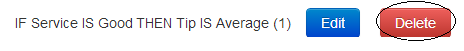
\includegraphics[width=0.45\textwidth]{images/test21.png}} }}\\ 
 \multicolumn{3}{l}{ }     \\\hline

Users can access help on how to create rules &  There will be a show help button, that when pressed, will display an explanation of the window & As Expected \\ 
  \hline
 \multicolumn{3}{c}{\fbox{ \raisebox{-\totalheight}{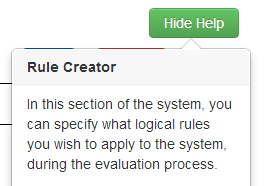
\includegraphics[width=0.3\textwidth]{images/test22.png}} }}\\ 
 \multicolumn{3}{l}{ }     \\\hline

Users will be able to edit the name of the system & There will be an input box to edit the name of the system & As Expected \\ 
  \hline
 \multicolumn{3}{c}{ \raisebox{-\totalheight}{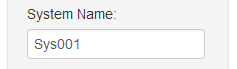
\includegraphics[width=0.3\textwidth]{images/test23.png}} }\\ 
 \multicolumn{3}{l}{ }     \\\hline

Users will be able to edit the type of evaluation to use &  There will be an input box to edit the type of the system & As Expected \\ 
  \hline
 \multicolumn{3}{c}{ \raisebox{-\totalheight}{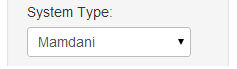
\includegraphics[width=0.3\textwidth]{images/test24.png}} }\\ 
 \multicolumn{3}{l}{ }     \\\hline

Users will be able to edit the ``and'' method to use &  There will be an input box to edit the ``and'' method of the system & As Expected  \\ 
  \hline
 \multicolumn{3}{c}{ \raisebox{-\totalheight}{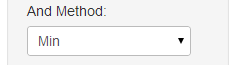
\includegraphics[width=0.3\textwidth]{images/test25.png}} }\\ 
 \multicolumn{3}{l}{ }     \\\hline

Users will be able to edit the ``or'' method to use & There will be an input box to edit the ``or'' method of the system & As Expected  \\ 
  \hline
 \multicolumn{3}{c}{ \raisebox{-\totalheight}{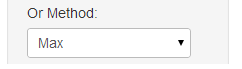
\includegraphics[width=0.3\textwidth]{images/test26.png}} }\\ 
 \multicolumn{3}{l}{ }     \\\hline

Users will be able to edit the aggregation method to use & There will be an input box to edit the aggregation method of the system &  As Expected \\ 
  \hline
 \multicolumn{3}{c}{ \raisebox{-\totalheight}{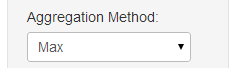
\includegraphics[width=0.3\textwidth]{images/test27.png}} }\\ 
 \multicolumn{3}{l}{ }     \\\hline

Users will be able to edit the implication method to use & There will be an input box to edit the implication method of the system & As Expected  \\ 
  \hline
 \multicolumn{3}{c}{ \raisebox{-\totalheight}{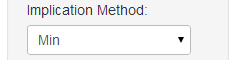
\includegraphics[width=0.3\textwidth]{images/test28.png}} }\\ 
 \multicolumn{3}{l}{ }     \\\hline

Users will be able to edit the defuzzification method to use & There will be an input box to edit the defuzzification method of the system &  As Expected \\ 
  \hline
 \multicolumn{3}{c}{ \raisebox{-\totalheight}{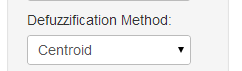
\includegraphics[width=0.3\textwidth]{images/test29.png}} }\\ 
 \multicolumn{3}{l}{ }     \\\hline

Users will be able to access help on what affect these changes make &  There will be a show help button, that when pressed, will display an explanation of the parameters & As Expected  \\ 
  \hline
 \multicolumn{3}{c}{ \raisebox{-\totalheight}{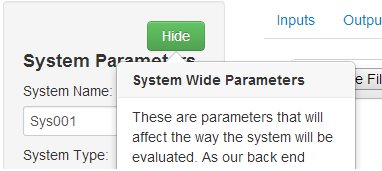
\includegraphics[width=0.4\textwidth]{images/test30.png}} }\\ 
 \multicolumn{3}{l}{ }     \\\hline

Users will be able to export their system as a MATLAB .fis file & On the export page, there will be an option to download a MATLAB .fis file & As Expected  \\ 
  \hline
 \multicolumn{3}{c}{ \raisebox{-\totalheight}{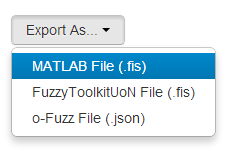
\includegraphics[width=0.3\textwidth]{images/test31.png}} }\\ 
 \multicolumn{3}{l}{ }     \\\hline

Users will be able to export their system as a FuzzyToolkitUoN .fis file & On the export page, there will be an option to download a FuzzyToolkitUoN .fis file & As Expected \\ 
  \hline
 \multicolumn{3}{c}{ \raisebox{-\totalheight}{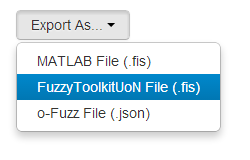
\includegraphics[width=0.3\textwidth]{images/test32.png}} }\\ 
 \multicolumn{3}{l}{ }     \\\hline

Users will be able to export their system as a JSON file & On the export page, there will be an option to download a JSON file &  As Expected \\ 
  \hline
 \multicolumn{3}{c}{ \raisebox{-\totalheight}{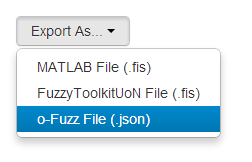
\includegraphics[width=0.3\textwidth]{images/test33.png}} }\\ 
 \multicolumn{3}{l}{ }     \\\hline

Users can access help on how to export files and what is supported &  There will be a show help button, that when pressed, will display an explanation of the window & As Expected \\ 
  \hline
 \multicolumn{3}{c}{\fbox{ \raisebox{-\totalheight}{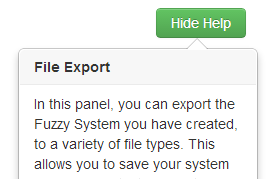
\includegraphics[width=0.3\textwidth]{images/test34.png}} }}\\ 
 \multicolumn{3}{l}{ }     \\\hline

Users will be able to import a MATLAB .fis file & Importing of MATLAB .fis files will be supported within the system & As Expected \\ 
  \hline
 \multicolumn{3}{c}{ \raisebox{-\totalheight}{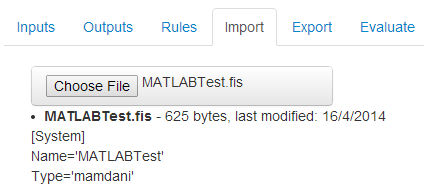
\includegraphics[width=0.5\textwidth]{images/test36.png}} }\\ 
 \multicolumn{3}{l}{ }     \\\hline

Users will be able to import a FuzzyToolkitUoN .fis file &  Importing of FuzzyToolkitUoN .fis files will be supported within the system & As Expected \\ 
  \hline
 \multicolumn{3}{c}{ \raisebox{-\totalheight}{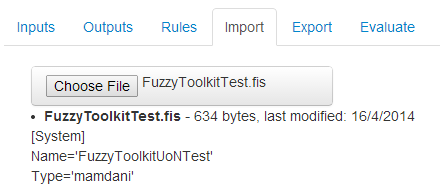
\includegraphics[width=0.5\textwidth]{images/test37.png}} }\\ 
 \multicolumn{3}{l}{ }     \\\hline

Users will be able to import a JSON file &  Importing of JSON files will be supported within the system & As Expected \\ 
  \hline
 \multicolumn{3}{c}{ \raisebox{-\totalheight}{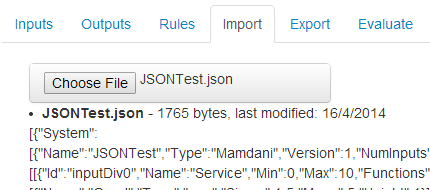
\includegraphics[width=0.5\textwidth]{images/test38.png}} }\\ 
 \multicolumn{3}{l}{ }     \\\hline

Users can access help on how to import files and what is supported &  There will be a show help button, that when pressed, will display an explanation of the window & As Expected \\ 
  \hline
 \multicolumn{3}{c}{\fbox{ \raisebox{-\totalheight}{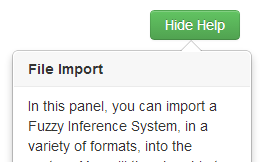
\includegraphics[width=0.3\textwidth]{images/test35.png}} }}\\ 
 \multicolumn{3}{l}{ }     \\\hline

Users can provide a value for each input, and receive the output value & An input box for each system input will be displayed, and an appropriate output displayed for each combination of input value provided  & As Expected \\ 
  \hline
 \multicolumn{3}{c}{\fbox{ \raisebox{-\totalheight}{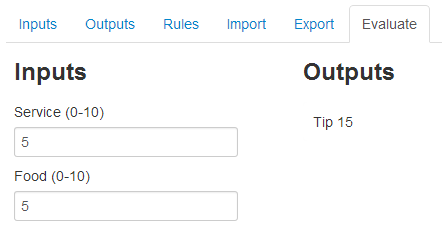
\includegraphics[width=0.4\textwidth]{images/test39.png}} }}\\ 
 \multicolumn{3}{l}{ }     \\\hline

Users can access help on how the evaluation process works &  There will be a show help button, that when pressed, will display an explanation of the window & As Expected \\
  \hline
 \multicolumn{3}{c}{ \raisebox{-\totalheight}{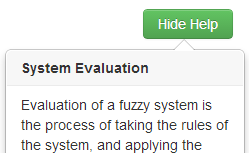
\includegraphics[width=0.3\textwidth]{images/test40.png}} }\\ 
 \multicolumn{3}{l}{ }     \\

  \end{longtable}